% !TEX root = ../thesis.tex
%
\chapter{Related Work}%
\label{sec:related}

Before Ohua, various other frameworks for parallel programming have been proposed that could serve as a replacement for \emph{Software Transactional Memory} in a shared state scenario to mitigate some of the shortcomings of the original proposal by Shavit et al.~\cite{shavit1997software}.
This chapter will briefly present some of this related work.

\section{Chocola: Combining multiple concurrency models}%
\label{sec:related:chocola}
According to Van Roy et al.~\cite{van2004concepts}, most concurrency models can be grouped into three different categories: deterministic, message-passing and shared memory models.
In a study, Swalens et al.~\cite{swalens2018chocola} found that developers often employ multiple concepts from different categories to solve their tasks.
They regard this interleaving of multiple concepts as highly dangerous, as each concurrency model comes with its own set of restrictions on what may or may not be done in the program in order to uphold their individual guarantees.
Mixing two or more models in an application may void some of these guarantees, a fact most developers are not aware of, as the semantics of this nesting are usually not well-defined.
For example, transactions (a shared-memory model) provide isolation\footnote{Isolation ensures, that one transaction can never see the changes made by another transaction until the latter has committed. Various levels of isolation have been defined, but Swalens et al.~\cite{swalens2018chocola} were only interested in serializability.} as a guarantee.
However, if futures (a deterministic model) are used inside of transactions, this guarantee is voided, unbeknownst to the developer.

As a solution, and to account for this culture of mixing several concurrency models, the authors propose \emph{Chocola}~\cite{swalens2018chocola}, a unified framework of futures, transactions and actors (a message-passing model).
Chocola is a fork of the Clojure programming language that comes with native support for all three concepts.
In their work, Swalens et al.\ provide well-defined semantics for the combination of two concurrency models.
When defining and implementing their language, they attempted to uphold as much of the original guarantees the individual models offered as possible when combining them, e.g., by altering how futures behave inside a transaction.
For the most part they succeeded, although determinacy was a guarantee they could often not retain.

To evaluate their work the authors also re-implemented a subset of the STAMP benchmark suite using Chocola.
However, they only tested 4 out of 8 benchmarks, as they argue that only the four selected ones offered any potential for enhancements by combining transactions with another concurrency model.
Swalens et al.\ reported speedups of 2.3 for a Chocola-based labyrinth implementation, as compared to a speedup of 1.3 for a conventional STM implementation.
Nevertheless, it remains unclear how the authors achieved these measurements, as this is not discussed in their work.
Judging from their references to previous work~\cite{swalens2016transactional, swalens2017transactional}, these speedups most likely refer to a single-threaded run of their STM implementation.
But as McSherry et al.~\cite{mcsherry2015scalability} pointed out in their work, choosing the performance of another implementation as reference point gives no indication of the real performance of both approaches.
In real application scenarios, parallelism is introduced to supercede an existing sequential implementation because the latter can usually only be optimized to a certain point before reaching its performance limit.
When setting a single-threaded run of any framework as baseline, one can only make a comparison between relative speedups to other frameworks, leading to distorted plots as can be seen in Fig.~\ref{fig:related:ohua-plots}.

\begin{figure}[t]
    \begin{subfigure}[t]{.48\textwidth}
        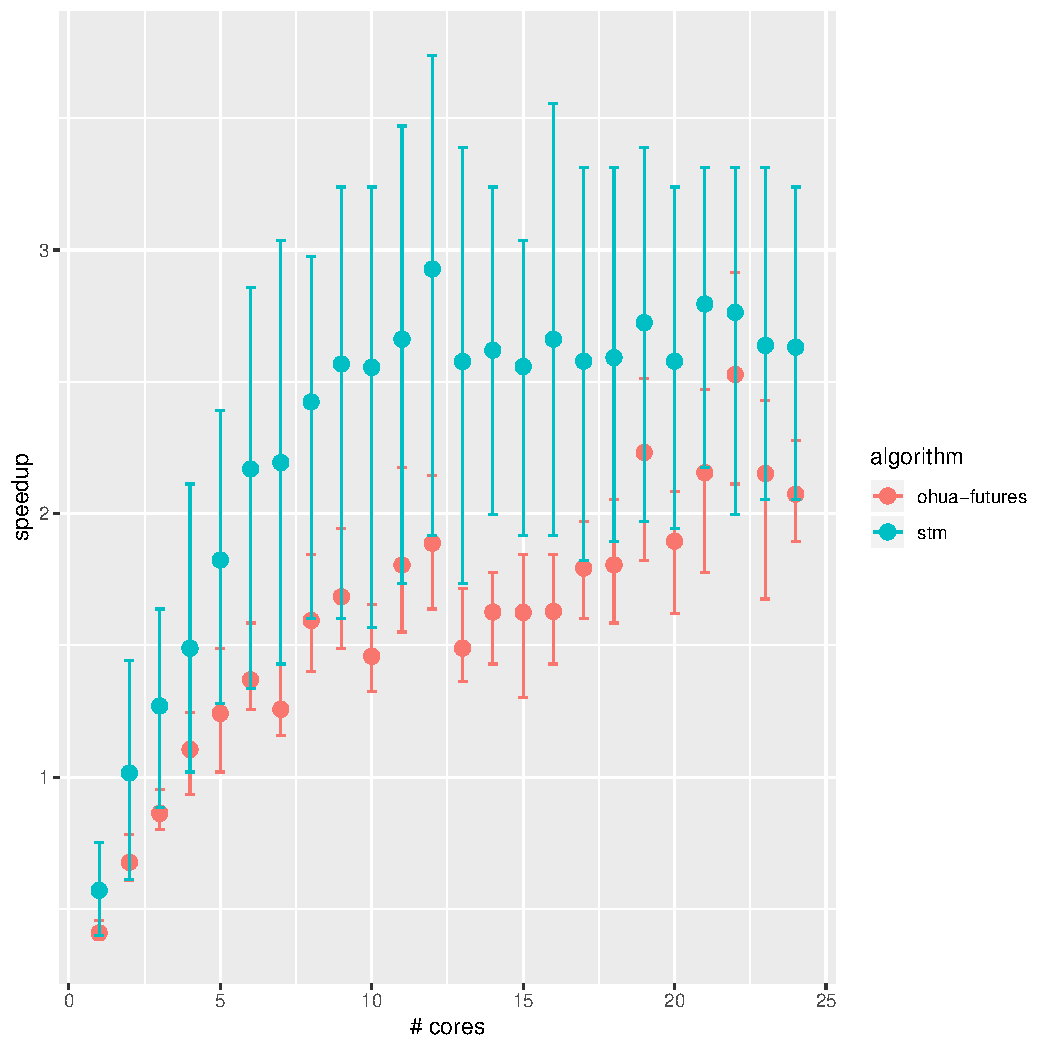
\includegraphics[width=\textwidth,keepaspectratio]{gfx/results/labyrinth/labyrinth+}
        \caption{Sequential baseline.}%
        \label{fig:related:ohua-plots:orig}
    \end{subfigure}
    ~
    \begin{subfigure}[t]{.48\textwidth}
        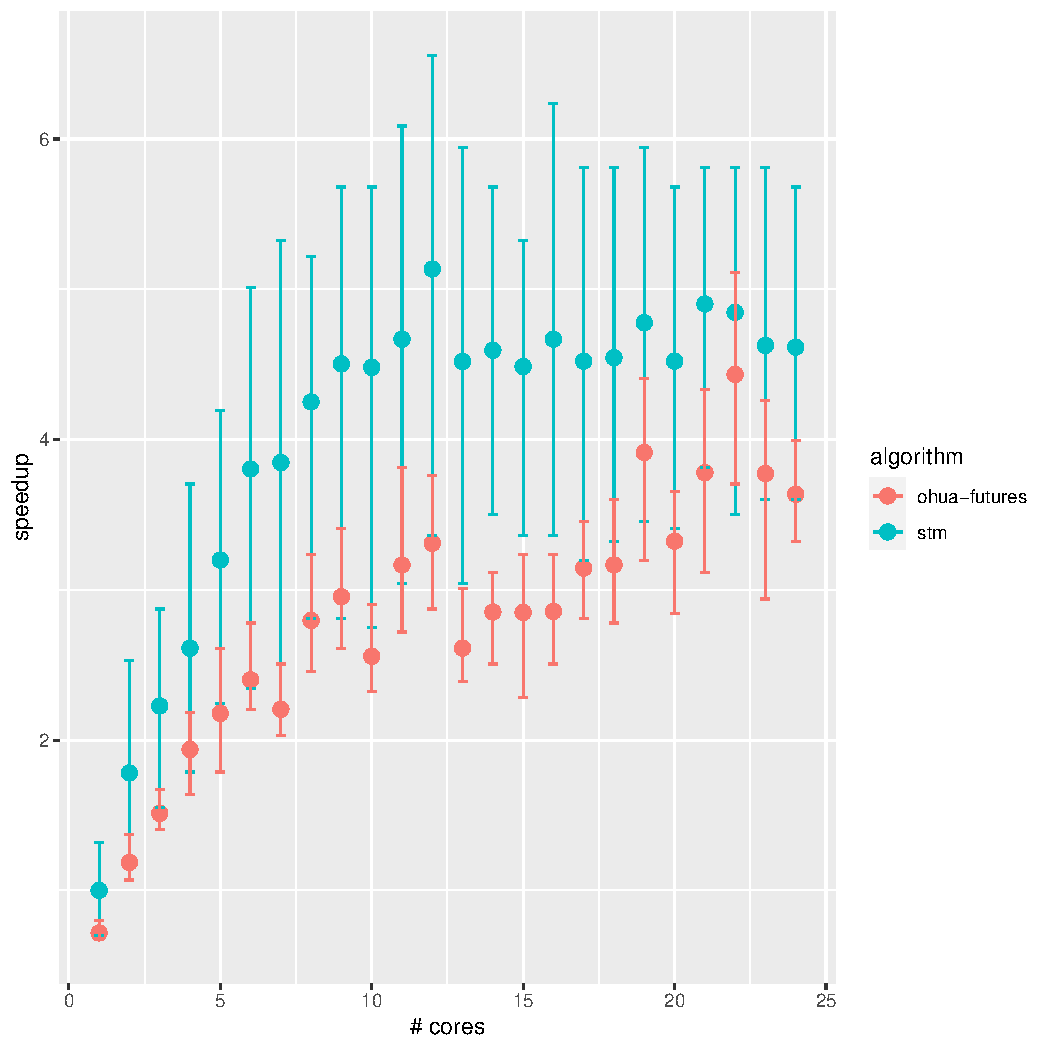
\includegraphics[width=\textwidth,keepaspectratio]{gfx/results/labyrinth/labyrinth+_stm_base}
        \caption{Single-threaded STM as baseline.}%
        \label{fig:related:ohua-plots:stm}
    \end{subfigure}
    \caption{Speedups of Ohua and STM for the labyrinth benchmark with different baselines.}%
    \label{fig:related:ohua-plots}
\end{figure}

Both plots show the results of the labyrinth+ benchmark as explained in Chapter~\ref{sec:experiments:labyrinth} and evaluated in Chapter~\ref{sec:evaluation:benchmarks}.
Figure~\ref{fig:related:ohua-plots:orig} shows our original speedups, comparing both implementations to a seuential baseline implementation.
Fig.~\ref{fig:related:ohua-plots:stm} on the other hand shows the same results but with the single-threaded STM run as baseline, nearly doubling the apparent speedups.
Hence, to obtain realistic speedups and account for the potential overheads of various frameworks, it is favorable to compare against a sequential baseline.
Swalens et al.\ probably decided against doing so as it would have required them to write a third, sequential version of their benchmarks.
This demonstrates another strength of Ohua: Due to its implicit nature, any algorithm definition may simultaneously serve as sequential implementation by simply executing the application as-is, without invoking the Ohua compiler first.
But due to this bad baseline choice, we cannot compare our results to those Chocola achieves.

A significant advantage of the authors' approach is, that it allows the combination of several different concurrency models while offering well-defined and formalized semantics.
This makes the development of complex software easier for developers as they do not have to put too much thought in the ramifications of this combination.
On the other hand side is this offering of multiple concurrency models also the frameworks' hugest disadvantage.
Developers now don't have to learn how to correctly use one, but three different concepts with different guarantees attached.
Resulting code is so extremely tailored towards the use of these different concepts and their interaction between one another that migrating the code to another framework becomes virtually impossible, depending on how many of Chocola's features are used.
Applications developed with this framework also contain many (potentially different) concurrency abstractions.
In that regard, developing parallel programs might become easier, but understanding and reasoning about them becomes much harder, especially compared to Ohua, which does not expose any abstractions and shields the developer completely from having to reason about concurrency, as this is exploited at compile-time.

\section{Software Lock Elision}%
\label{sec:related:sle}
Roy et al.~\cite{roy2009runtime} detail in their work the problems of migrating lock-based code to a Transactional Memory framework.
If done incorrectly, the semantics of the code may change due to the different behavior of transactions compared to locks, leading to different results.
Hence, they propose a Software Lock Elision runtime that builds upon lock-based code and allows threads to speculatively execute lock-based critical sections in parallel.
This framework features an optimistic execution model and detects conflicts between accesses by concurrent threads dynamically.
In this regard, it functions similar to Software Transactional Memory.
But additionally, Software Lock Elision takes a best effort approach on its implementation:
A fallback to acquiring locks without any speculation is possible, e.g., when the speculative state overflows the cache, when using nested locks or when performing an operation that only works non-speculatively (such as waiting for a condition variable).
Roy et al.\ state that their system is only tailored towards workloads with high contention and a low number of conflicts, as only then using locks becomes a liability, producing too much overhead.

\begin{figure}
    \centering
    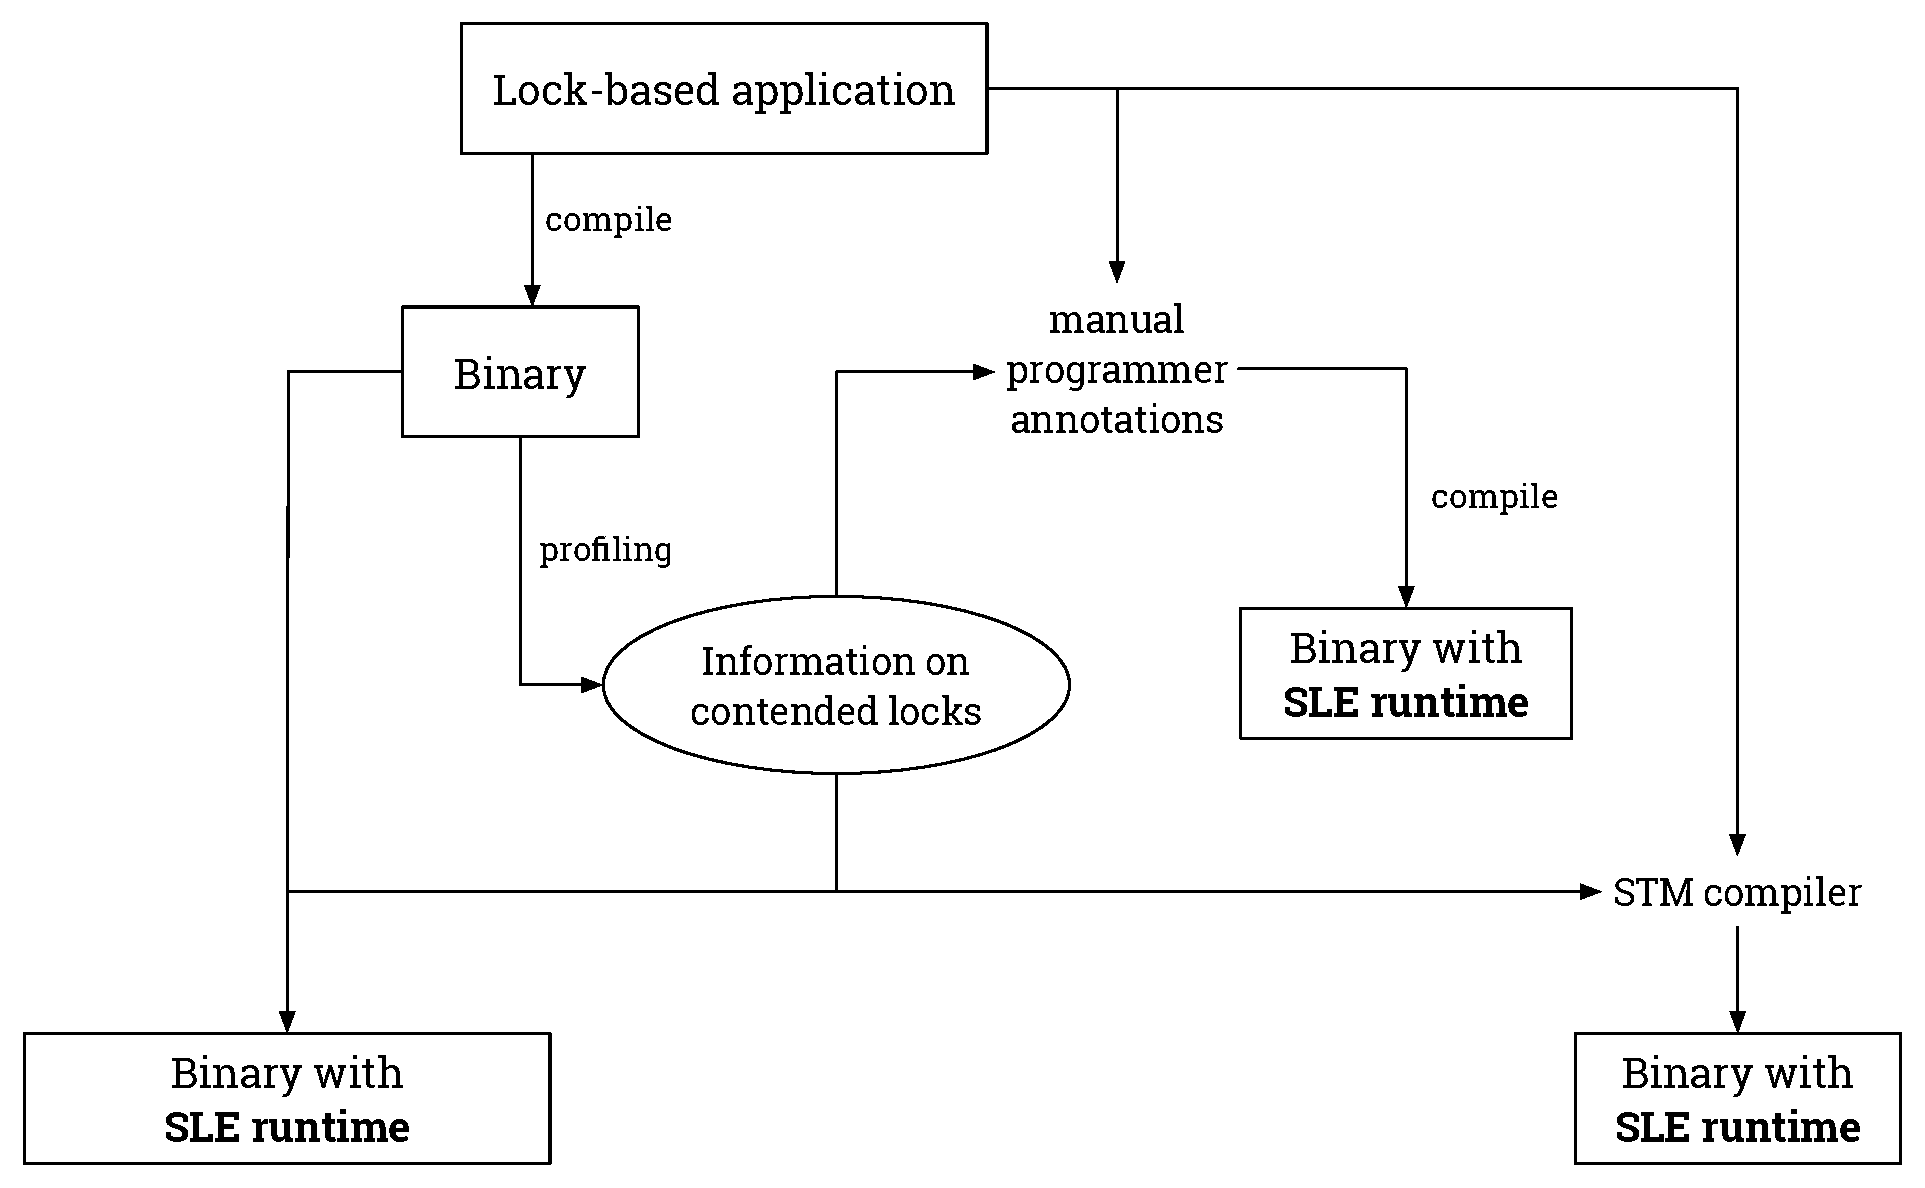
\includegraphics[width=.9\textwidth,keepaspectratio]{gfx/related/sle}
    \caption{The workflow of the Software Lock Elision runtime. Adapted from Roy et al.~\cite{roy2009runtime}.}%
    \label{fig:related:sle}
\end{figure}

As can be seen in Fig.~\ref{fig:related:sle}, their design features both the automatic and the manual use of SLE.
A developer may either annotate her lock-based code to explicitly use Software Lock Elision at certain points or profile the locks in her binary and apply binary rewriting systems to add a SLE runtime to the application\footnote{In their work, Roy et al.\ discuss the design for an automated SLE runtime but left an actual implementation to future work. As of today, no follow-up work detailing an actual implementation has been provided.}.
The runtime is designed to retain maximal fairness towards non-speculative locks by prioritizing them over threads holding the same lock speculatively.
The authors also tried to ensure the isolation between speculative and non-speculative work and to add support for application-specific lock types.

To evaluate their work, Roy et al.\ implemented 6 out of 8 STAMP benchmarks\footnote{They reported 2 benchmarks, \emph{yada}~\& \emph{bayes}, to not run on their systems anymore.} using manually-annotated SLE code.
For the \emph{kmeans}, \emph{intruder} and \emph{ssca2} benchmarks the authors reported speedups 1.5 to 2 times higher than those of the original STM implementation.
However, the SLE runtime failed to achieve good results for \emph{genome}, \emph{labyrinth} and \emph{vacation}, sometimes only reaching 25-50~\% of the STM speedup.
Interestingly, the framework only achieved good performances in benchmarks with short transactions and at most a medium amount of time spent in transactions, as can be seen in table~\ref{tab:experiments:categorization}.

Overall, this type of automated approach to enhance lock-based code with speculation looks very promising.
It allows the use of STM concepts within lock-based code, which enables developers to easily improve performance of their existing code.
But this requires the use of lock-based code.
The authors make the correct usage of locks a prerequisite in their work, although this is the hardest aspect of lock-based programming, as we discussed in Chapter~\ref{sec:background:stm}.
Therefore, an abstraction-free approach to concurrent programming, like Ohua, might be preferable to avoid having developers write locking code manually.

\section{Heterogeneous Parallelism}
\label{sec:related:manticore}
Fluet et al.~\cite{fluet2007manticore} argue, that currently, no parallel programming language exists, that can be adequately used for general purpose programming, as most of these languages are tailored towards research purposes.
Additionally, they lament the missing parallelism features in general purpose programming languages.
In their opinion, parallel languages need to provide mechanisms for multiple levels of parallelism, since most applications exhibit parallelism at multiple levels that could be exploited for performance and since most commodity hardware achieves optimal performance only when exploiting these multiple parallelism levels (e.g., by employing both threads and SIMD parallelism).
In response, the authors propose \emph{Manticore}~\cite{fluet2007manticore, fluet2007status, fluet2009programming, fluet2010implicitly}, a parallel language for heterogeneous parallelism.

The language belongs to the family of statically-typed strict functional languages and bases its concurrency mechanisms on Concurrent ML.
Coarse-grain parallelism in Manticore is achieved using explicit mechanisms like \texttt{spawn} for thread creation and typed channels.
An important feature of the language is the absence of shared state.
Instead, threads may only use message passing via aforementioned channels for communication and synchronization.
As opposed to coarse-grain parallelism, the fine-grain parallelism is achieved using implicit mechanisms, because Fluet et al. argue that this type of parallelism is cumbersome to implement by hand and can easily pose large overheads when done incorrectly.
For this, they use constructs like parallel arrays (immutable sequences that can be computed in parallel), which are all created or invoked using special annotations.

\begin{listing}[h]
    \begin{minted}{SML}
        fun imgToGray img =
            [: [: rgbToG pix | pix in row :]
                | row in img :]
        fun convert img = let
            val replCh = channel()
            in
                spawn (send (replCh, imgToGray img));
                recvEvt replCh
            end
    \end{minted}
    \caption{Code example showcasing implicit and explicit parallelism in Manticore, adapted from~\cite{fluet2007manticore}.}%
    \label{fig:related:manticore}
\end{listing}

Listing~\ref{fig:related:manticore} features parallel comprehension syntax as an example for such annotations in the function \texttt{imgToGray}, also showing that these parallel list comprehensions can also be nested.
The function \texttt{convert} on the other hand shows the use of explicit parallelism for coarse-grain parallelism.
To efficiently harness the resulting parallel code, Manticore includes a continuation-based runtime that caters to the different scheduling needs of explicit and implicit threads.

Although Fluet et al.\ have been continuously working on Manticore and published several follow-up works, no benchmarks have been conducted with the language yet.
Nonetheless is the author's proposition very interesting as it is also relying on finding and extracting implicit parallelism, like Ohua.
Unfortunately, they only employ this idea for lower-level parallelism, leaving much of the parallelization effort to the developer, who may not be able to parallelize the code as efficient as automated approaches.
Another shared approach with Ohua is the elimination of shared state, by which many types of errors in parallel code can be ruled out.


\section{Flexible Parallel Execution}%
\label{sec:related:parcae}
The approach that is perhaps the most similar to Ohua's approach is \emph{Parcae}~\cite{raman2012parcae} by Raman et al.
Like us, they opted for an automatic approach for their work, eliminating the need for explicitly managing threads.
Though, their motivation lies within the fact that most parallelization efforts target only a static, anticipated number of environments, outside which a programs performance may decrease drastically.
Parcae was designed to circumvent that issue by allowing it to automatically tune the program dynamically to react to any changes in the environment at runtime.

\begin{figure}[h]
    \centering
    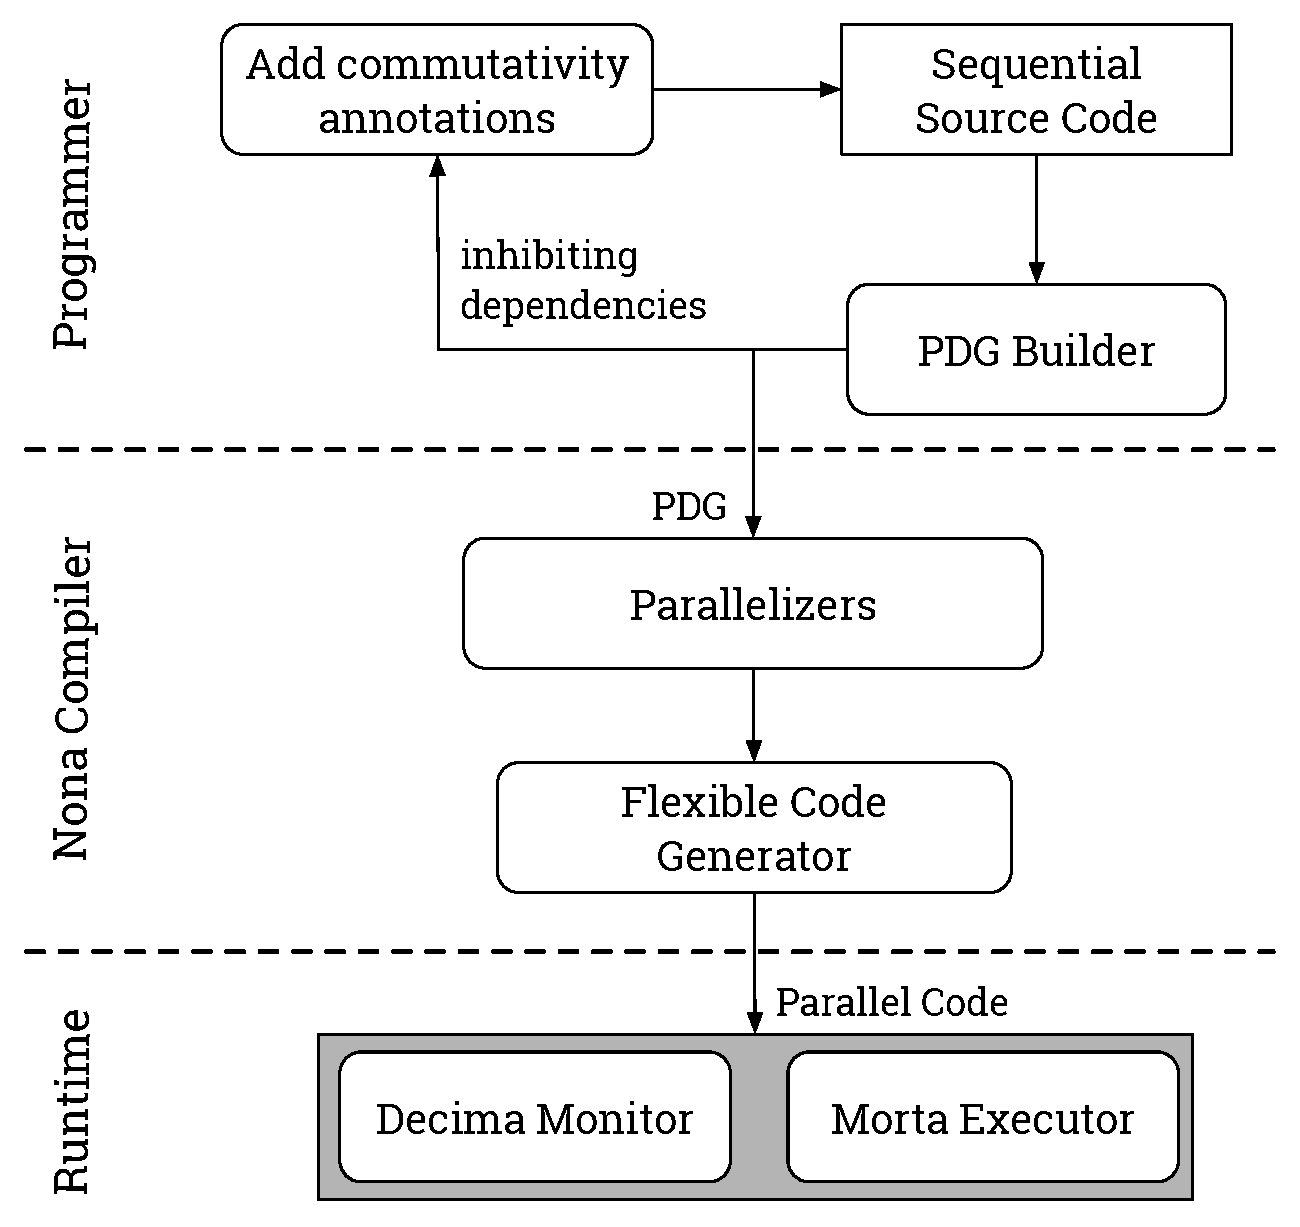
\includegraphics[width=.6\textwidth,keepaspectratio]{gfx/related/parcae}
    \caption{Architecture and Workflow of the Parcae framework, adapted from~\cite{raman2012parcae}.}%
    \label{fig:related:parcae}
\end{figure}

These flexible parallel programs, as the authors call them, are generated by the Nona compiler, one of the three components comprising the Parcae framework, which is shown in Fig.~\ref{fig:related:parcae}.
The compiler takes a sequential program as input and identifies parallelizable regions within it by building a program dependence graph, to which some node reordering and regrouping operations are applied, which might require further annotations from the developer to highlight commutative operations.
It then applies the parallelizing transforms to reach of these regions, although currently only loop nests are in scope for this step.
Such transformations encompass data-parallel transforms with critical sections and pipeline transforms but developers may expand this list at their choosing.
Nona then creates several tasks, each containing a loop body, which are marked either for parallel or sequential execution.
The resulting program contains numerous hooks for profiling and a set of tasks which are to be executed.
At runtime, the Morta executor takes care of executing the program and finding a parallelism configuration that is optimal for the execution environment.
This happens by first executing a sequential version of the parallel regions and monitoring the execution using the third component, the Decima Monitor.
Based on the gathered information, the execution scheme of the program is adjusted to optimize performance, which becomes a continuous process throughout execution. %the whole execution.

To evaluate their work, Raman et al.\ chose applications from a variety of benchmark suites and implemented them using Parcae.
In the \emph{kmeans} benchmark, which was chosen as representative from the STAMP suite, Parcae was able to improve performance by about 42 \% compared to a baseline parallel execution while only consuming 84 \% of the power a baseline parallel implementation consumed.

When comparing Parcae with Ohua, one can find many similarities in the languages approaches, although the initial motivation behind both concepts is different.
One of the most prominent differences between both frameworks on the other hand is that Parcae requires much scheduler knowledge and has a high degree of dynamicity in the runtime, imposing non-negligible overheads during execution, which the authors also acknowledged.
Ohua solves most of these issues as compile time by creating a runtime where data dependencies dictate when a tasks has to be executed sequentially or whether a parallel execution with other operators is possible.
For scheduling, we currently mostly rely on the Operating System scheduler, avoiding costly reconfigurations at runtime.
Also, we do not require annotations of any sort in the source code, but rather deduce all necessary information from the Data Flow Graph.
While we do not achieve as good performance improvements for the \emph{kmeans} application, we manage to only use about 5-20 \% of the CPU time STM uses, indicating higher energy savings than reported for Parcae.
